\documentclass{article}

% Language setting
% Replace `english' with e.g. `spanish' to change the document language
\usepackage[english]{babel}

% Set page size and margins
% Replace `letterpaper' with `a4paper' for UK/EU standard size
\usepackage[letterpaper,top=2cm,bottom=2cm,left=3cm,right=3cm,marginparwidth=1.75cm]{geometry}

% Useful packages
\usepackage{amsmath}
\usepackage{graphicx}
\usepackage{float}
\usepackage{svg}
\usepackage{graphicx,wrapfig,lipsum}
\usepackage{listings}
\usepackage{enumitem}
\usepackage{mathtools}
\usepackage[dvipsnames]{xcolor}
\usepackage{optidef}
\newcommand\mat[1]{\mathcal{#1}}
\definecolor{verylightgrey}{RGB}{236, 236, 236}
\usepackage[colorlinks=true, allcolors=blue]{hyperref}


\usepackage{blindtext}
\title{Deep Learning Boosted Markowitz Model for Portfolio Construction}
\author{Rodrigo Cepeda Marín}

\begin{document}



\maketitle
\begin{figure}[H]
\begin{center}
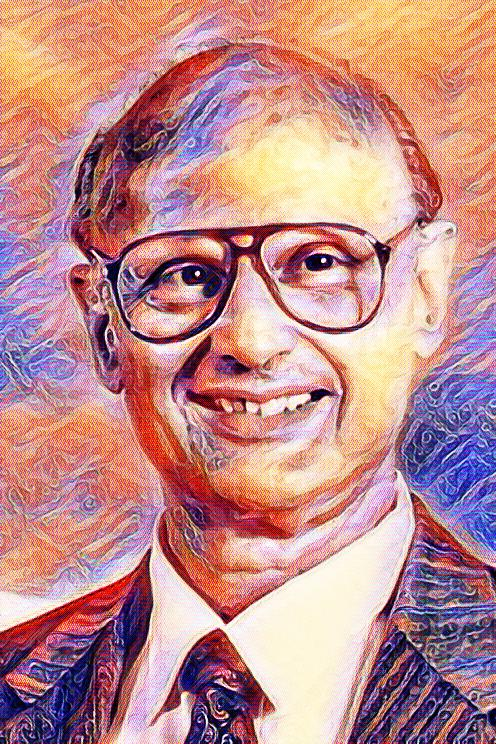
\includegraphics[width=0.6\linewidth]{Plots/marko.jpg}

\end{center}
\end{figure}

\clearpage

\section{Introduction}
\label{intro}
The Markowitz model, one of the best-known portfolio construction models, takes into account an important assumption: future returns on assets are known based on recent past returns.

This paper evaluates the possibility of using complex deep learning structures to estimate asset correlation and therefore asset covariance, one of the inputs that feed the Markowitz model, to reduce the impact of this initial assumption. The structure of the work will be as follows:
\begin{enumerate}
    \item First, the Modern Portfolio Theory will be presented along with the traditional Markowitz model \textit{t-Marko}.
    \item Next, a deep learning model will be introduced and explained to estimate future asset correlation.
    \item Third, the investment universe will be presented and used to train the deep learning model.
    \item The fourth chapter will compare the results between the \textit{t-Marko} model and the Markowitz model using the previously estimated future correlation, \textit{boost-Marko}.
    \item Finally, the conclusions and possible future work will be presented.
\end{enumerate}


\section{The Modern Portfolio Theory}
The Modern Portfolio Theory (MPT), formulated in 1952 by the economist Harry Markowitz, addresses the finding of the optimal portfolio that can be constructed with a set of assets by minimizing the risk, measured in terms of volatility, for every expected return. The portfolios with the greater return for every possible volatility generate the efficient frontier.

Under the MPT, the risk and return of the portfolio is respectively calculated as:
\begin{equation}
    \sigma_{p}^{2} = \sum_{i}^{n}\sum_{j}^{n}{w_{i}\sigma_{i,j}w_{j}} = w \times Cov \times w^{T}
\end{equation}
\begin{equation}
    \mu_{p} = \sum_{i=1}^{n}{w_{i} \mu_{i}}
\end{equation}

where $w_{i} \in [0,1]$ is the weight of each asset in the portfolio and $\sum_{i = 1}^{n}{w_{i}} = 1$, $Cov \in \mat{A}_{n,n}$ and $\times$ represents matrix multiplication.



In 1966, Sharpe applied a risk-reward ratio to evaluate the performance of a given portfolio known as the Sharpe Ratio:
\begin{equation}
    S_{p} = \frac{\mu_{p} - r}{\sigma_{p}}
\end{equation}
The portfolio with the greater Sharpe ratio, the optimal portfolio, is located in the efficient frontier and can be found by solving the following minimization problem:

\begin{mini!}|l|[3]
{}{-\frac{\sum_{i=1}^{n}{w_{i} \mu_{i}}}{\sqrt{w\times Cov \times w^{T}}}}
{}{}
\addConstraint{\sum_{i}^{n}{w_{i}} = 1}
\addConstraint{w\in[0,1]}{}
\end{mini!}

As per described above, the portfolio with the highest Sharpe ratio, the optimal portfolio using the Markowitz model, can be found with three inputs:
\begin{enumerate}[label=(\textbf{\alph*})]
    \item The vector of $w$, i.e., $w_{i}$ such that $ 0\leq w_i \leq 1$, $\sum_{i}{w_i}=1$ $\forall$ $i \in {1,...,n}$ 
    \item The vector of $\mu$, i.e., $\mu_{i}$ such that $i \in {1,...,n}$
    \item The covariance matrix $Cov_{i,j}$ such that $i,j \in {1,...,n}$ 
\end{enumerate}


As mentioned in \ref{intro}, the finding of the optimal portfolio using \textit{t-Marko} is based on the assumption that past returns imply future returns, therefore the next step will be to describe a methodology to forecast certain model inputs and transit from \textit{t-Marko} to \textit{boost-Marko}.


\section{Deep Learning Model}
This section will describe a deep learning model that estimates future asset correlations $Corr_{i,j}$ based on past observed ones. The covariance will be then calculated as: $$Cov_{i,j} = Corr_{i,j}\sigma_{i}\sigma_{j}$$
Where $\sigma_{i}$ is the observed standard deviation for asset $i$.


\begin{wrapfigure}{Hr}{6cm}
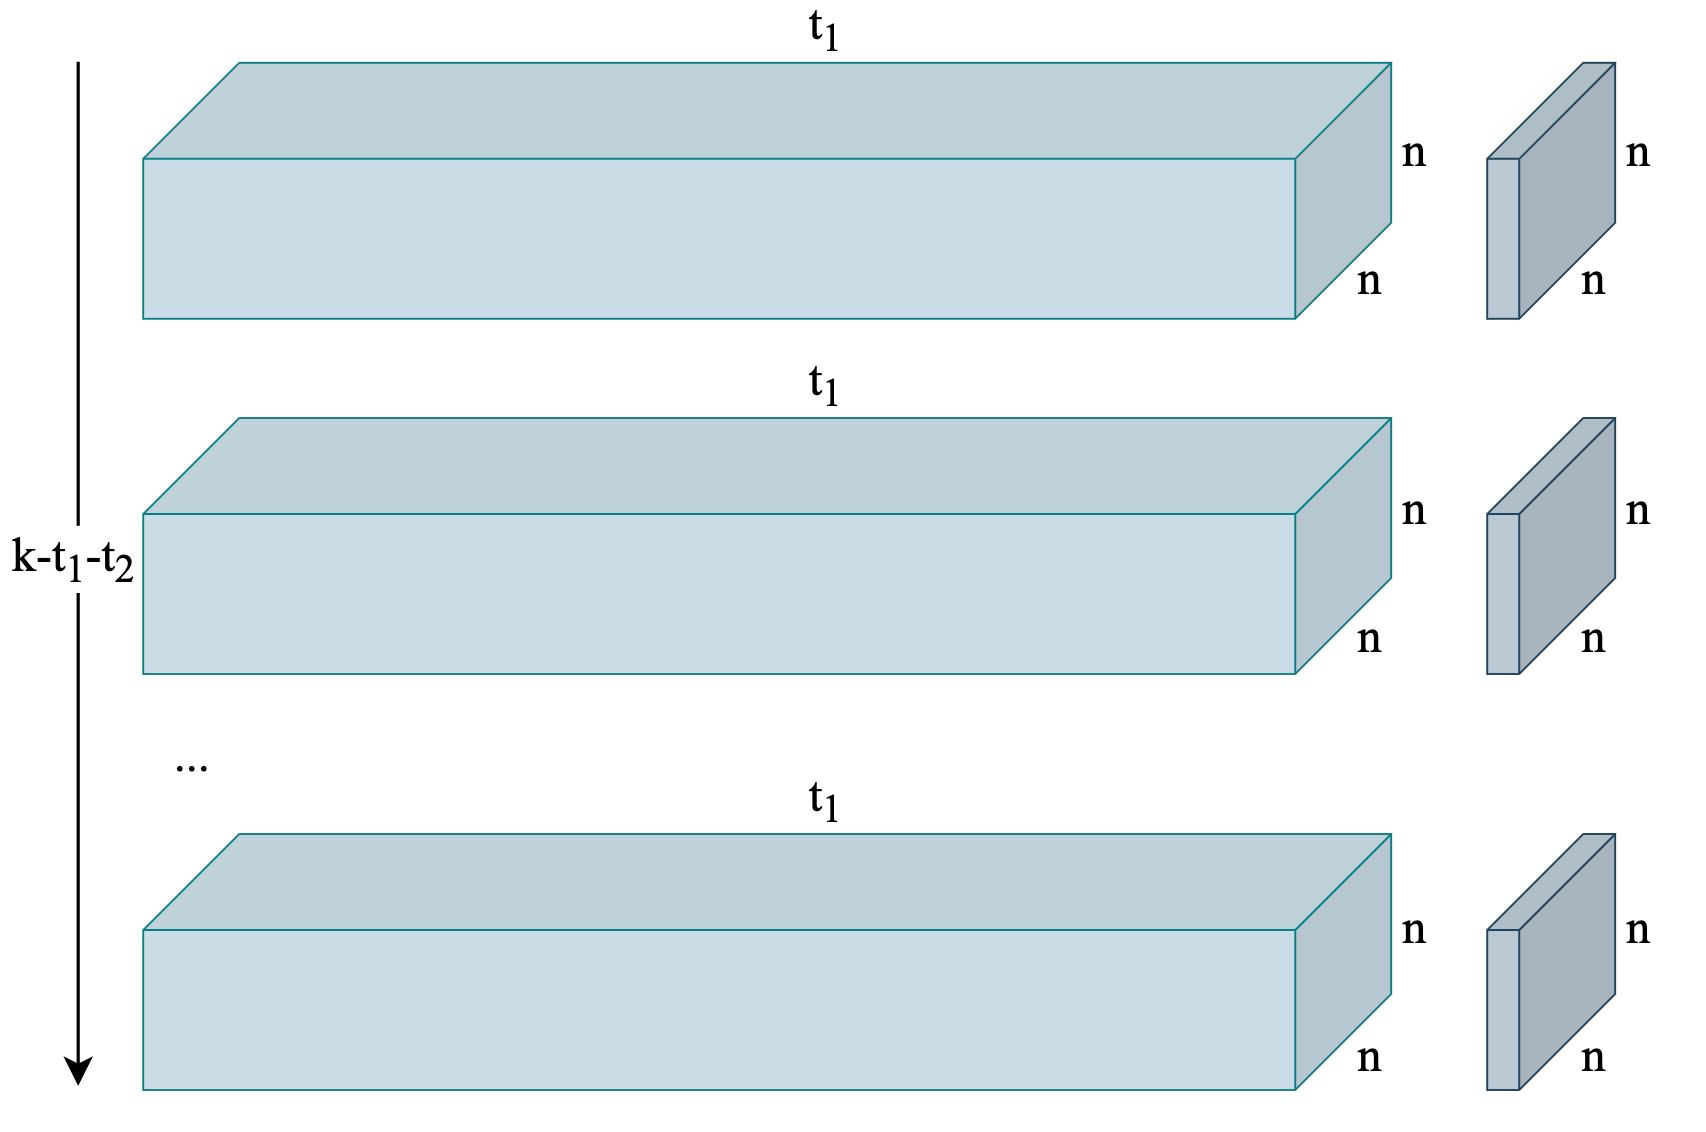
\includegraphics[width=1\linewidth]{Plots/Diagram_v3.png}
\caption{$Corr$ cubes structure}\label{wrap-fig:1}
\end{wrapfigure}
First, it is important to understand the nature and shape of the information that is to be predicted: The correlation matrix $Corr \in \mat{A}_{n,n}$ is a symmetric matrix with $n$ rows and columns, being $n$ the number of assets in out portfolio, with $a_{i,i} = 1$ $\forall$ $i \in n$ and where the value $a_{i,j} = a_{j,i}$ $\forall$ $i,j \in n$ describes the correlation between assets $i$ and $j$.

With a set of $k$ returns for all the assets we could build $k-t_{1}$ matrices where $t_{1}$ is the window of returns used to calculate each correlation matrix. 

Finally, we have a temporal structure of $k-t_{1} - t_{2}$ matrices which we are going to use for predicting the future correlation values, where $t_{2}$ is the amount of correlation matrices used to predict the $t + 1$ correlation matrix. The final structure is as presented below:

As seen in Figure \ref{wrap-fig:1}, the two factors contained in the information that need to be captured, along with the architecture used for that task are:
\begin{enumerate}
    \item The two-dimensional relationship between the data in the correlation matrix, which will be captured using a convolutional neural architecture
    \item The sequential nature of each correlation in time, which will be captured using a recurrent neural archirecture
\end{enumerate}

\subsection{Convolutional Neural Networks}
\textit{Among different deep learning architecture, a special type of multilayer neural network for spatial data is the Convolutional Neural Network (CNN).}
\begin{flushright}\small
(\cite{ghosh2020fundamental})
\end{flushright}
CNN are very commonly used to train image shaped information by making use of convolutions, which are multidimensional operations of a fixed size performed in the the entire input that capture internal relations. The architecture of a CNN is inspired by the visual systems of living beings and will be used in the network proposed in this paper to analyze the two-dimensional structure in the correlation matrix. A convolution can be graphically represented with the following graph:
\begin{figure}[H]
\begin{center}
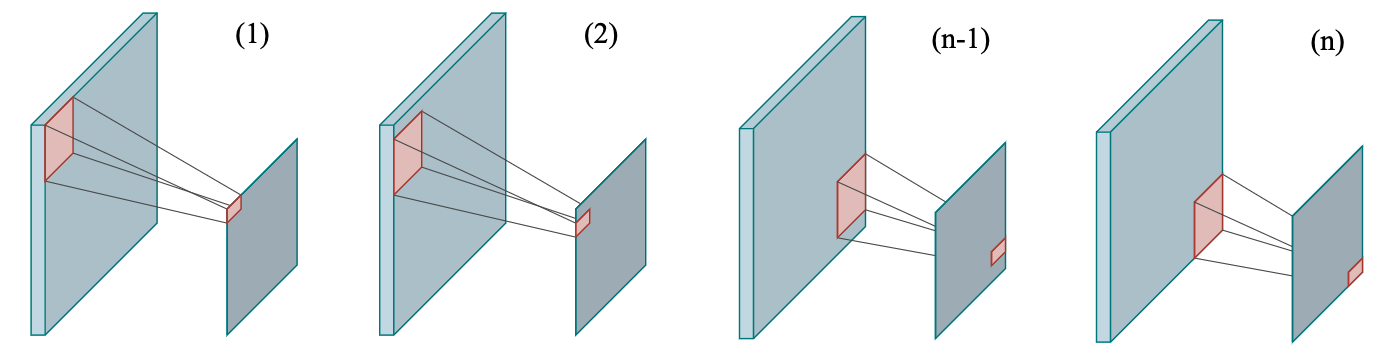
\includegraphics[width=0.75\linewidth]{Plots/Convo2.png}
\caption{Representation of a convolution in a 2D matrix}
\end{center}

\end{figure}
If $Corr_{i,j,t}$ is treated as a $(n,n)$ image, where $a_{i,j} \in Corr_{i,j,t}$ is represented in the scale of grays, one layer and a convolution on it would look like explained in the following graph: 

\begin{figure}[H]
    \centering
{{
\includegraphics[width=0.45\textwidth]{Plots/Corr.png} }}%
    \qquad
{{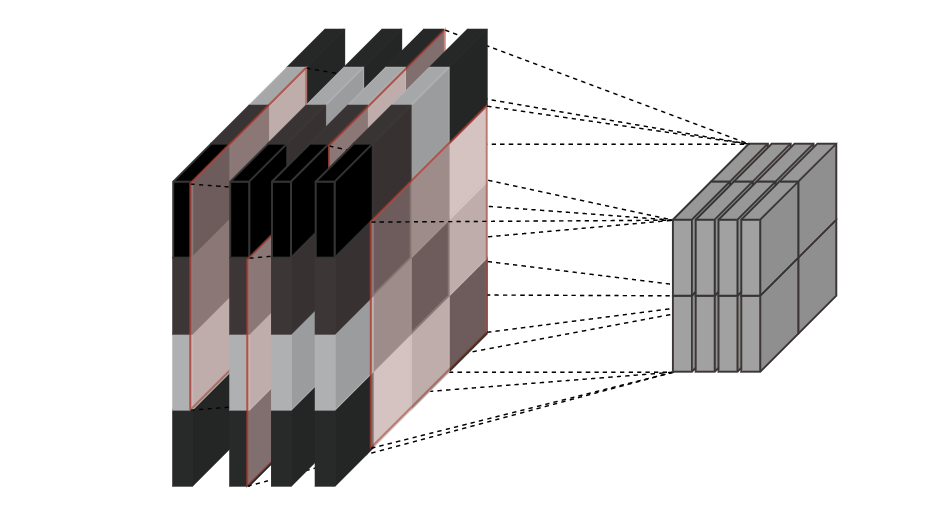
\includegraphics[width=0.45\textwidth]{Plots/Corr_v1.png} }}%
    \caption{$Corr$ matrix on the left and $(3,3)$ convolution on a $Corr$ matrix on the right}%
\end{figure}



\subsection{Recurrent Neural Networks}

\begin{wrapfigure}{HL}{3cm}
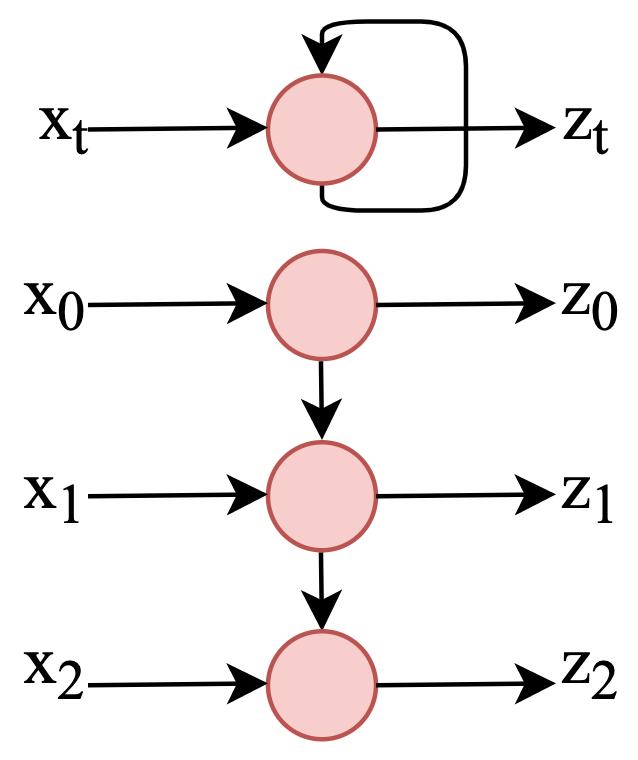
\includegraphics[width=1\linewidth]{Plots/RNN2.png}
\caption{RNN}\label{wrap-fig:2}
\end{wrapfigure}



\textit{Recurrent Neural Networks (RNN) are networks capable of modelling sequential data for sequence recognition and prediction. RNNs are made of high dimensional hidden states with non-linear dynamics. The structure of hidden states work as the memory of the network and state of the hidden layer at a time is conditioned on its previous state. This structure enables the RNNs to store, remember, and process past complex signals for long time periods.}
\begin{flushright}\small
(\cite{salehinejad2017recent})
\end{flushright}

RNNs have a main problem: their instability due to exploding and vanishing gradients. A model specifically designed to tackle this problem is the long-short term memory networks (LSTM), presented in 1997 in \cite{hochreiter1997long}. LSTMs are a kind of RNN that controls the flow of information to hidden neurons and preserve extracted features from previous time steps while avoiding the vanishing and exploding gradient problem.



The use of this networks will allow the model to capture the sequential information contained in the asset correlation time series. For example the historical correlation between Iberdrola, Sacyr and ACS can be seen below:

\begin{figure}[H]
    \centering
{{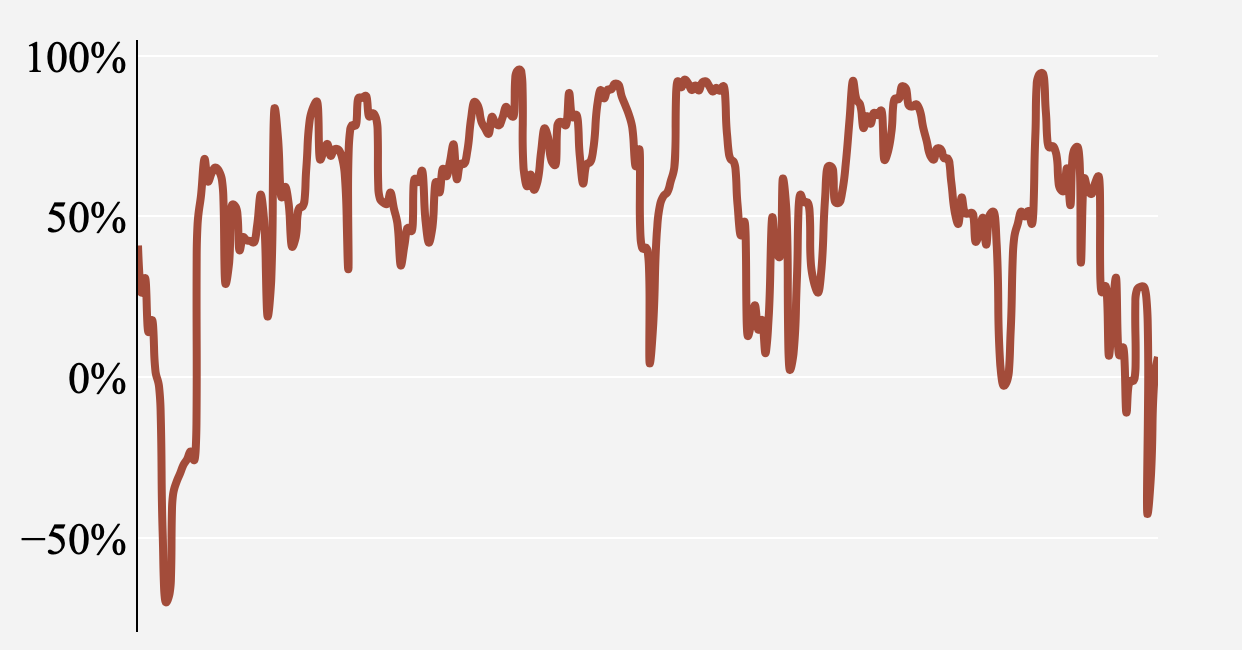
\includegraphics[width=0.45\textwidth]{Plots/corr31.png} }}%
    \qquad
{{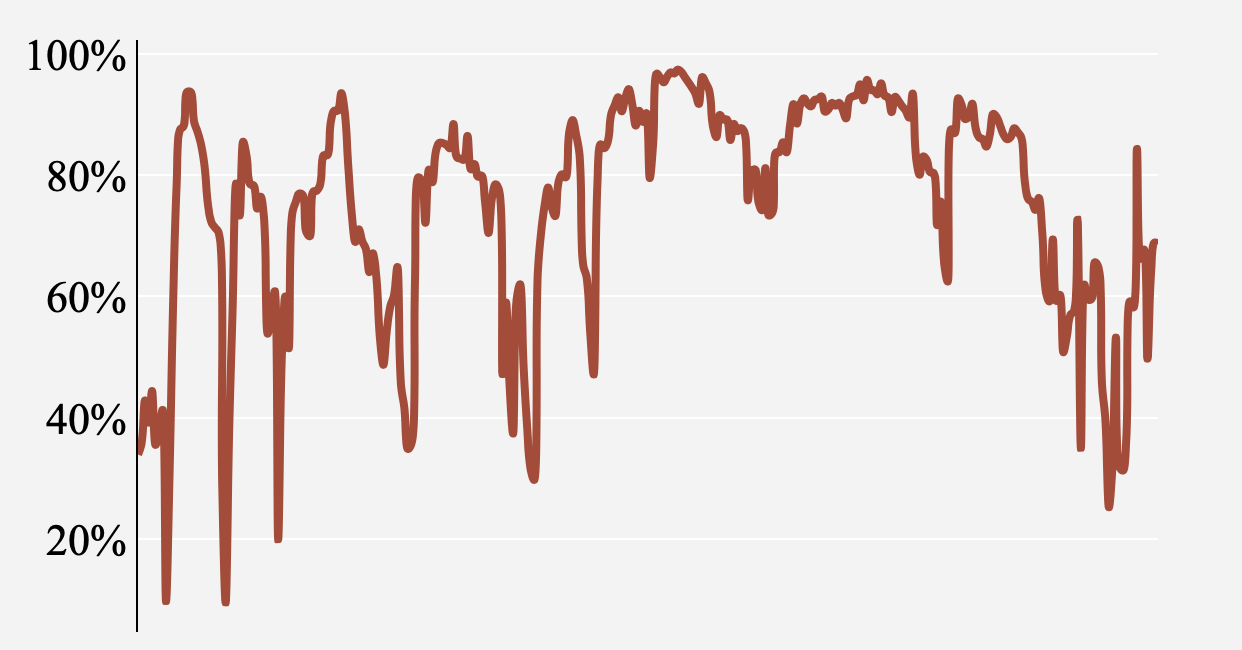
\includegraphics[width=0.45\textwidth]{Plots/corr32.png} }}%
    \caption{IBE.MC-SCYR.MC correlation on the left and IBE.MC-ACS.MC correlation on the right}%
\end{figure}

\subsection{ConvLSTM}
The two architectures presented are constructed to deal with image shaped and sequential data respectively. The combination of both, presented in \cite{shi2015convolutional} as ConvLSTM, will be the main pillar used in the deep learning model used to forecast future correlation matrices.

The ConvLSTM model was first presented to forecast precipitations in a certain area based on satellite images. Even though this application might seem far apart from the goal of this paper, the main idea behind the forecasting is the same: A set $\mat{S}$ of images, is analyzed to forecast the weather in certain area. The relationships between the pixels of the image are important to understand, since the aggregation of them form the shapes that the model is looking for, and the time development of the images is also a key factor, since the state of set $\mat{S}_{t}$ depends on the state of $\mat{S}_{t-1}$.
\section{Model Construction and Training}

Up to this point, the document has described:
\begin{enumerate}
    \item An investment strategy for our portfolio which maximises the Sharpe ratio using three inputs \textit{observed in the past}; the assets mean returns $\mu_{i}$ $\forall i\in[0,n]$, the assets standard deviations $\sigma_{i}$ $\forall i\in[0,n]$ and the covariance between assets.
    \item A deep learning model family that is able to forecast $n$-dimensional outputs with the use of the temporal relations implied in the input information.
\end{enumerate}

From this point on, this two lines of work converge, and the goal of the document will be to describe the process of constructing and rebalancing a portfolio using the Markowitz model mixing observed and  predicted market information; the \textit{boost-Marko}. As per described in section 2, the \textit{boost-Marko} model takes three inputs:
\begin{enumerate}[label=(\textbf{\alph*})]
    \item $\sigma_{i}$ such that $i \in {1,...,n}$, which will continue to be observed past information.
    \item $\mu_{i}$ such that $i \in {1,...,n}$,  which will continue to be observed past information.
    \item The covariance matrix $Cov_{i,j}$ such that $i,j \in {1,...,n}$, which will be derived from the future $Corr_{i,j}$ matrix estimated. $Cov_{i,j} = Cov_{i,j}\sigma_{i}\sigma_{j}$
\end{enumerate}

The next subsection will describe the investment universe considered for this paper as well as the restrictions for the construction of portfolios. After that, the models will be constructed and trained for each possible portfolios and the results will be presented in \ref{sec5}.
\subsection{Investment Universe}
Let $\mat{U}$ be the investment universe for this study, which consists on ten of the top companies present in the Spanish IBEX35 index. The ticker (Yahoo Finance API) and name of the assets is specified below:
\begin{center}
\begin{tabular}{ |c|c|} 
\hline
 \textbf{Ticker} & \textbf{Name}\\ 
 \hline
 IBE.MC & Iberdrola, S.A.\\ 
 \hline
 ITX.MC & Industria de Diseño Textil, S.A.\\
 \hline
 SAN.MC & Banco Santander, S.A.\\
 \hline
 TEF.MC & Telefónica, S.A.\\ 
 \hline
 REP.MC & Repsol, S.A.\\
 \hline
 BBVA.MC & Banco Bilbao Vizcaya Argentaria, S.A. \\
 \hline
 SCYR.MC & Sacyr, S.A. \\
 \hline
 MEL.MC & Meliá Hotels International, S.A. \\
 \hline
 ACS.MC & Actividades de Construcción y Servicios, S.A. \\
 \hline
 IAG.MC & International Consolidated Airlines Group S.A. \\
 \hline
\end{tabular}
\end{center}


Let $\mat{P}$ be the portfolio that is intended to be created. It is defined that $\mat{P}$ is constructed of five assets $p_{i} \in \mat{U}$ and will be rebalanced every 10 trading days.

For each day $t$, $\mu_{p_{i}, t} = \sum_{h=t-1}^{t-10}{r_{p_{i}, h}}$ where $r$ is the logistic return and the volatility is calculated as the 10 day standard deviation for each asset.

According to the Combination formula, a total of $\frac{10!}{4!\,(10-4)!} = 210$ different portfolios can be built using the available assets in the investment universe.

\subsection{Model Construction}


To obtain the predicted correlation matrix for the 210 portfolios, we can proceed in two separate ways:

\begin{enumerate}
    \item First, to train the entire investment universe and subset the correlations for each portfolio. This way, the training is performed on a $(t, n, n)$ matrix where $n = 10$.
    \item Second, to obtain the correlation for each portfolio by training a model where the inputs contains information only on the assets included. This way 210 different models are trained using $(t, 5, 5)$ matrices. 
\end{enumerate}

The second methodology is more expensive computationally but it's more accurate as well. The simpler and smaller matrices allow the model to understand better the relationships between past correlations between each asset. This is the approach that will be taken to continue the investigation

A snippet of the Python code to create model $\mat{M}_{m}$ where $m \in [0, 210]$ can be seen below:
\lstinputlisting[backgroundcolor = \color{verylightgrey}, language=Python]{Code/Model.py}

\subsection{Model Train}
The models have been trained using Google Colab's GPU. Each of them is constructed by more than 700.000 parameters and has been trained for 50 epochs using a 0.001 learning rate on an Adam optimizer.

Each model has generated a $(29, 5 ,5)$ matrix containing the estimated correlations. Using that information alongside the past observed volatility $\sigma_{i}$, the covariance matrix $Cov_{i,j,t}$ for each time step and every portfolio is obtained. This matrix will feed \textit{boost-Marko} while the historical $Cov_{i,j,t}$ matrix will feed \textit{t-Marko}.



\section{Deep Learning Boosted Markowitz}
\label{sec5}
In this section the performance of the \textit{t-Marko} model will be compared with the performance of the deep learning boosted Markowitz model. The metric used to compare performances will be the mean of the 10-day Sharpe ratio along all the rebalancings in the lifespan of each portfolio.  

For each of the 210 portfolios, the algorithm has rebalanced 28 times, between 2021-05-24 and 2022-06-24 every 10 trading days. Some information is presented below:

\begin{center}
\begin{tabular}{ |c|c|c|} 
\hline
 \textbf{Metric} & \textbf{Original} & \textbf{Predicted}\\ 
 \hline
 Minimum Sharpe & -0.965 & -1.083\\ 
 \hline
 Maximum Sharpe & 1.187 & 0.809\\ 
 \hline
 Mean Sharpe & -0.044 & 0.002\\ 
 \hline
 \end{tabular}
\end{center}



\begin{wrapfigure}{Hr}{7.5cm}
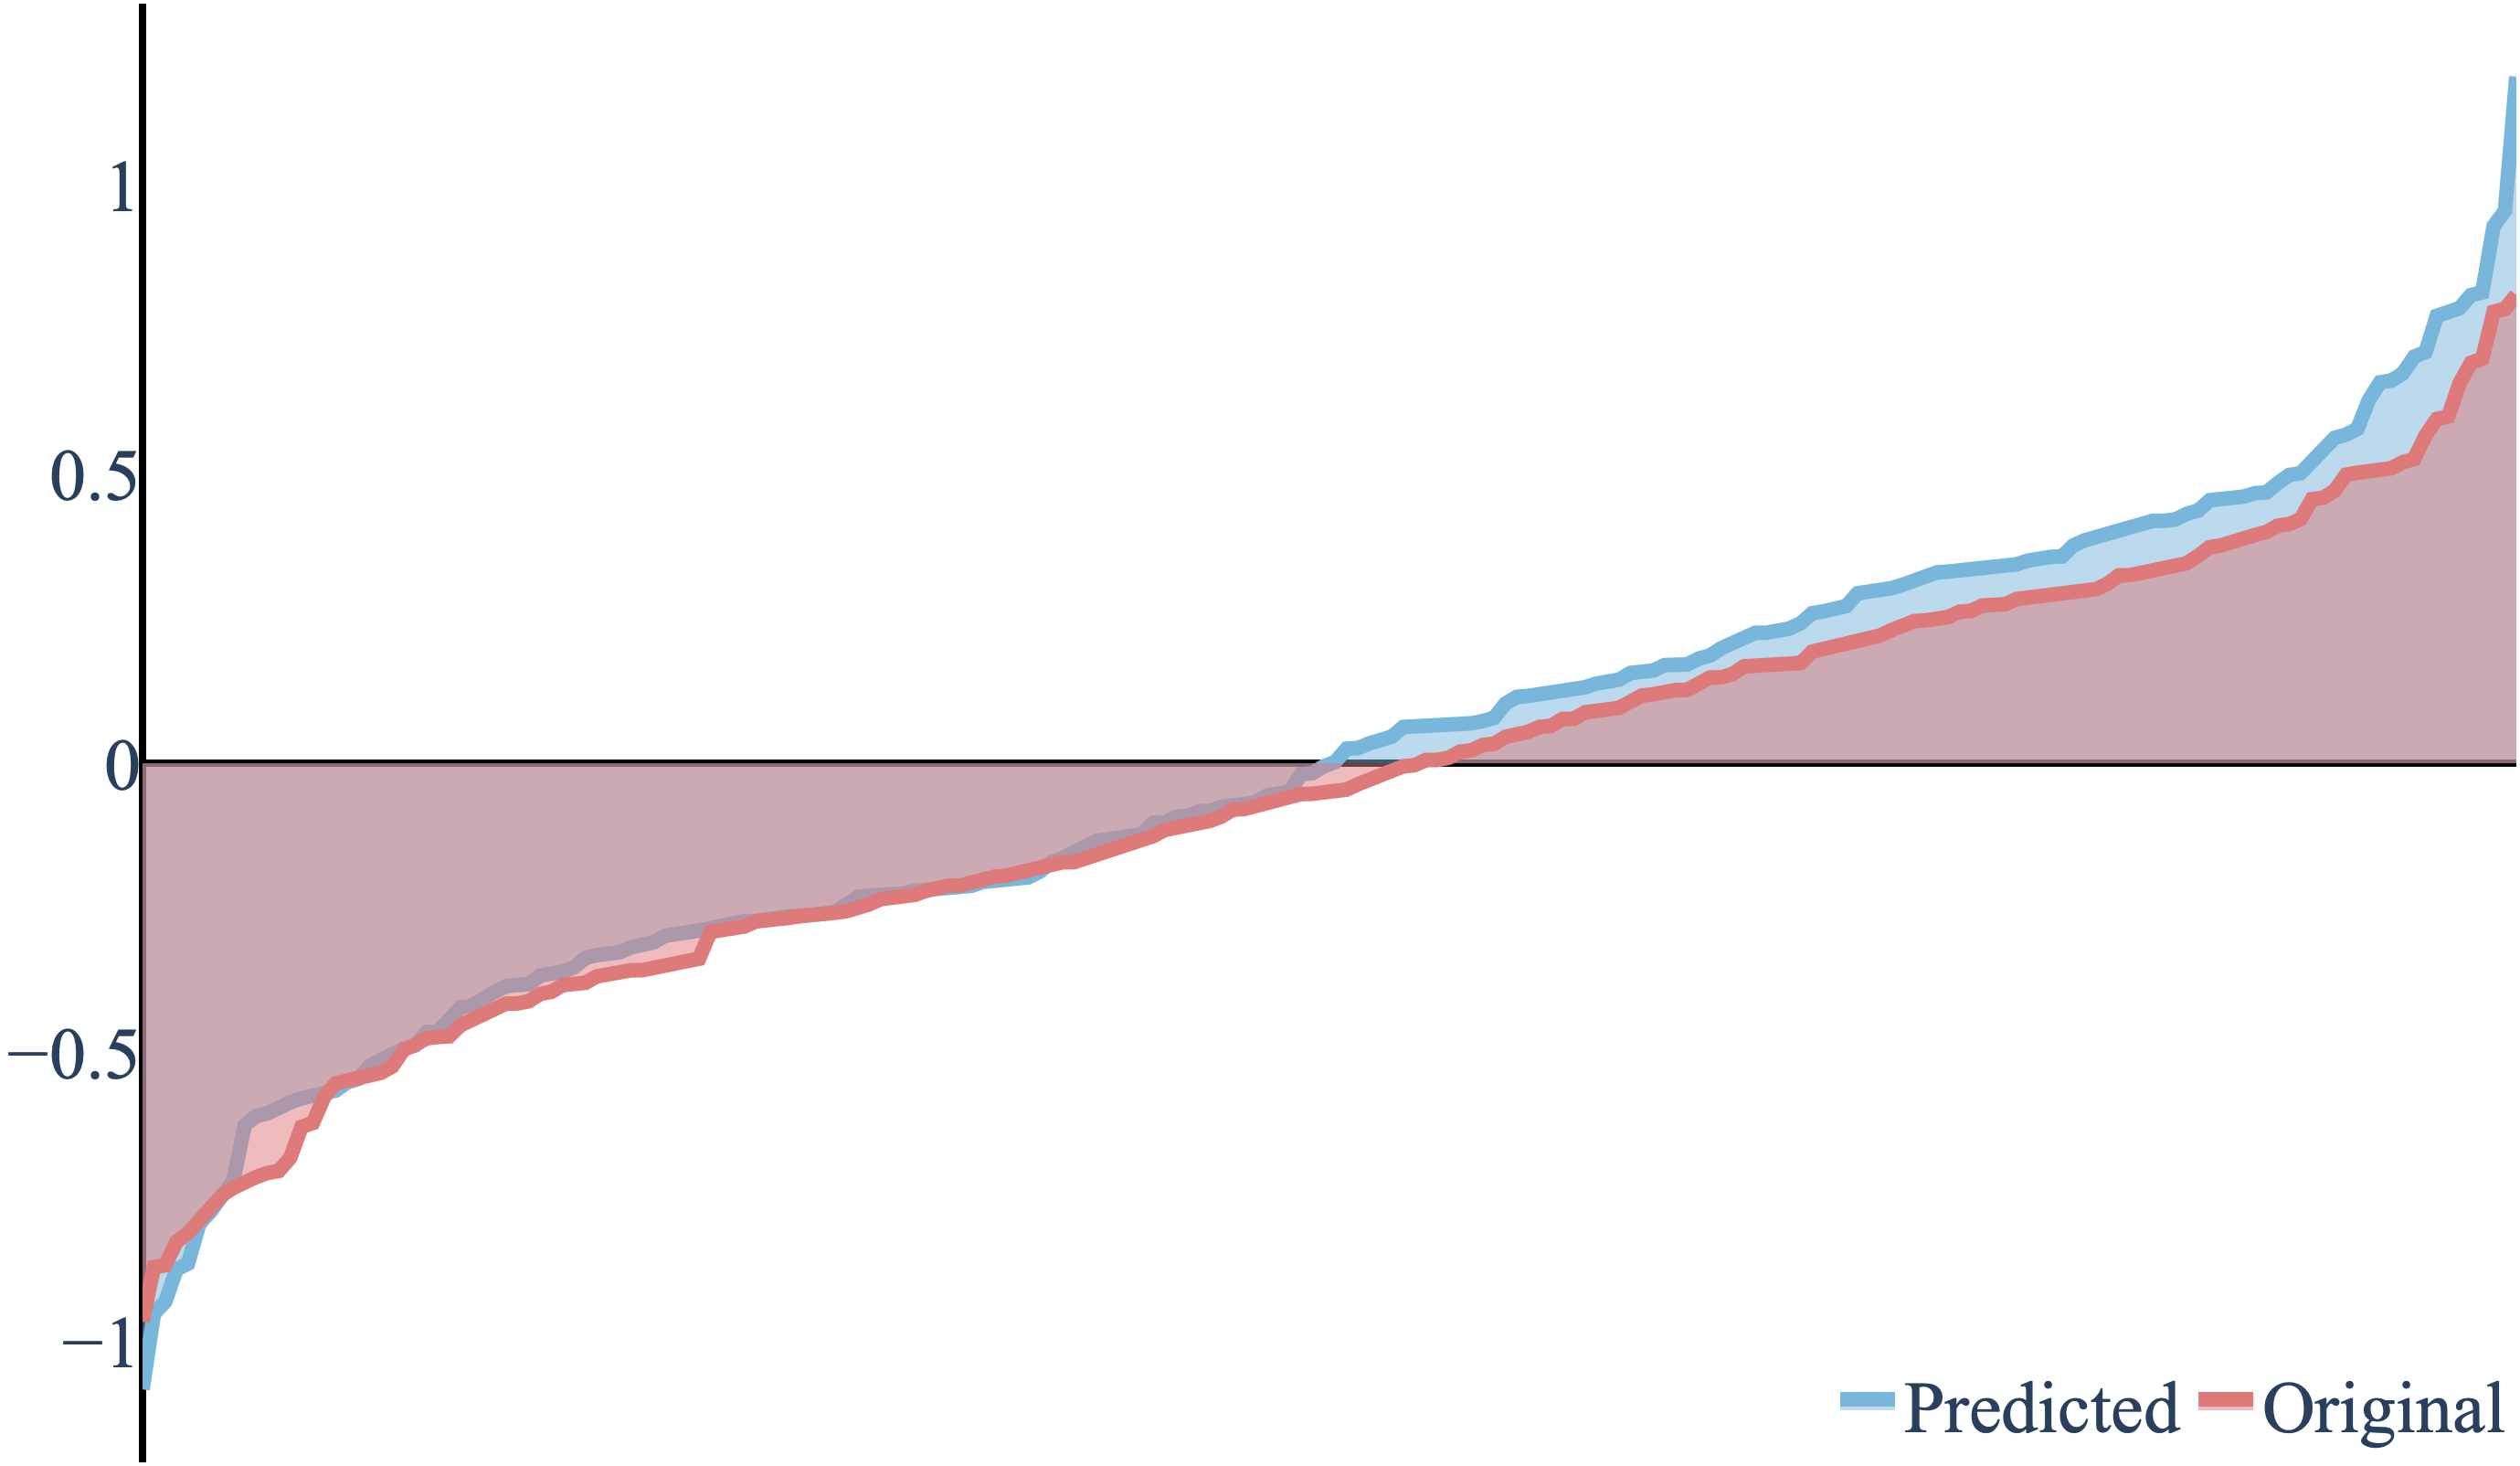
\includegraphics[width=1\linewidth]{Plots/shorder.png}
\caption{Sorted Sharpe values for both models}\label{wrap-fig:2}
\end{wrapfigure}

135 out of the 210 portfolios, a \textbf{64.28\%} of them, have a greater mean Sharpe ratio along their entire duration when using the deep learning predicted correlation matrix $Corr_{i,j}$ than when using the past observed one.

The Mean Squared Error (MSE) mean value for the validation sets of all 210 portfolios is 6\%, while if the MSE for the non trained correlation matrices, i.e., the MSE of $Corr_{i,j,t}$ and $Corr_{i,j,t-1}$ $\forall t$ is calculated, the value obtained is above 10\%.

92\% of the portfolios for which the MSE in the validation training set is smaller than 10\% have a greater Sharpe ratio with the deep learning boosted Markowitz model than with the original Markowitz model, which shows that the validations MSE being below 10\% and the success of the deep learning model are strongly correlated.

It is also interesting to see that the rebalancings that differ between both models are less than a third of the total. From the 5880 total rebalancings, 28 per portfolio for 210 portfolios, only 1890 are different, which is a 32.14\%. 

Out of the 1890 rebalancings that differ, the outcome of 55.5\% of them is translated into a greater Sharpe, but most importantly, the rebalancings that perform better, have a greater spread between both Sharpe ratios than the rebalancings that perform worse.

\begin{center}
\begin{tabular}{ |c|c|c|} 
\hline
 \textbf{Metric} & \textbf{Positive} & \textbf{Negative}\\ 
 \hline
 Rebalances & 1050 & 840\\ 
 \hline
 Percentaje of total & 55.5\% & 45.5\%\\
 \hline
 Total Sharpe & 1133.00 & -565.68\\ 
 \hline
 Mean Total Sharpe  & 1.079 & -0.672\\ 
 \hline
 \end{tabular}
\end{center}

\subsection{Simulation Analysis}
To understand the size and periodicity of the changes in the asset weights between both models, a certain portfolio is analyzed. The portfolio composed by IBE.MC, BBVA.MC, MEL.MC and ACS.MC, (the first simulated portfolio) has a mean original Sharpe ratio of 0.247 and a mean predicted one of 0.344. Let this portfolio be analysed to see the difference in the allocations along time.
First the weight composition of the portfolio depending on the training strategy:
\begin{figure}[H]
    \centering
{{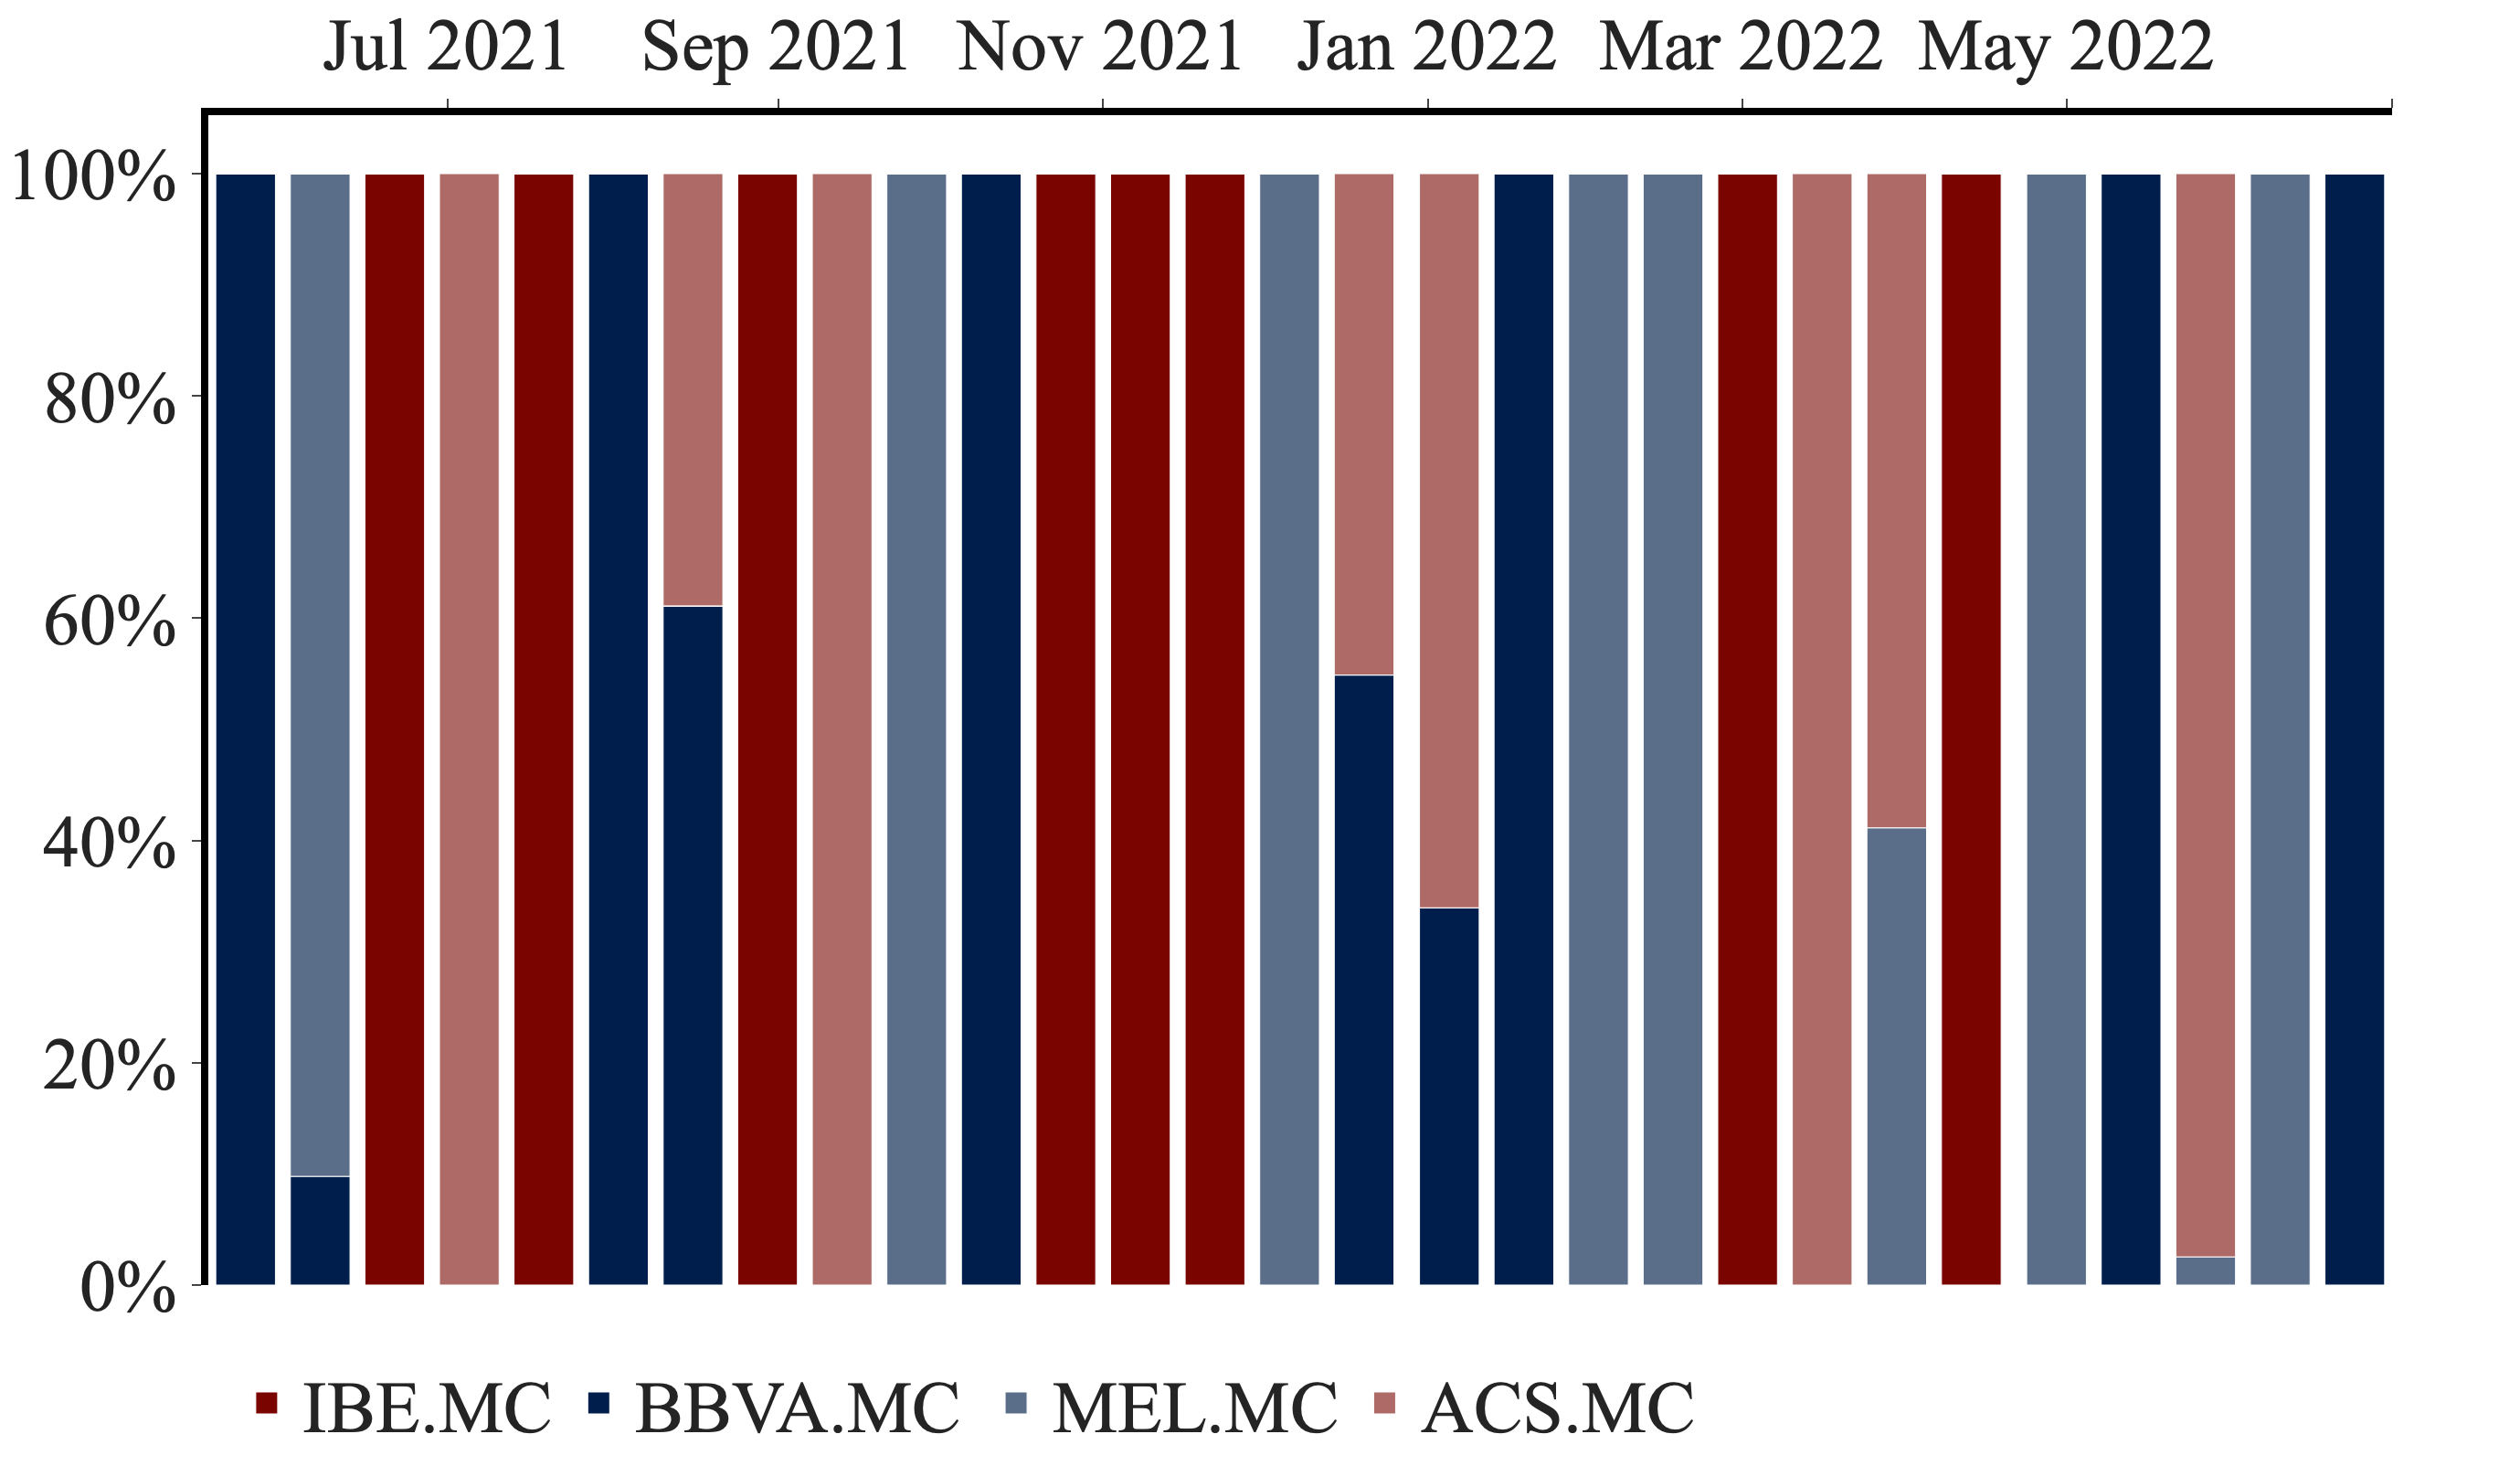
\includegraphics[width=0.4\textwidth]{Plots/w_or.png}}}%
    \qquad
{{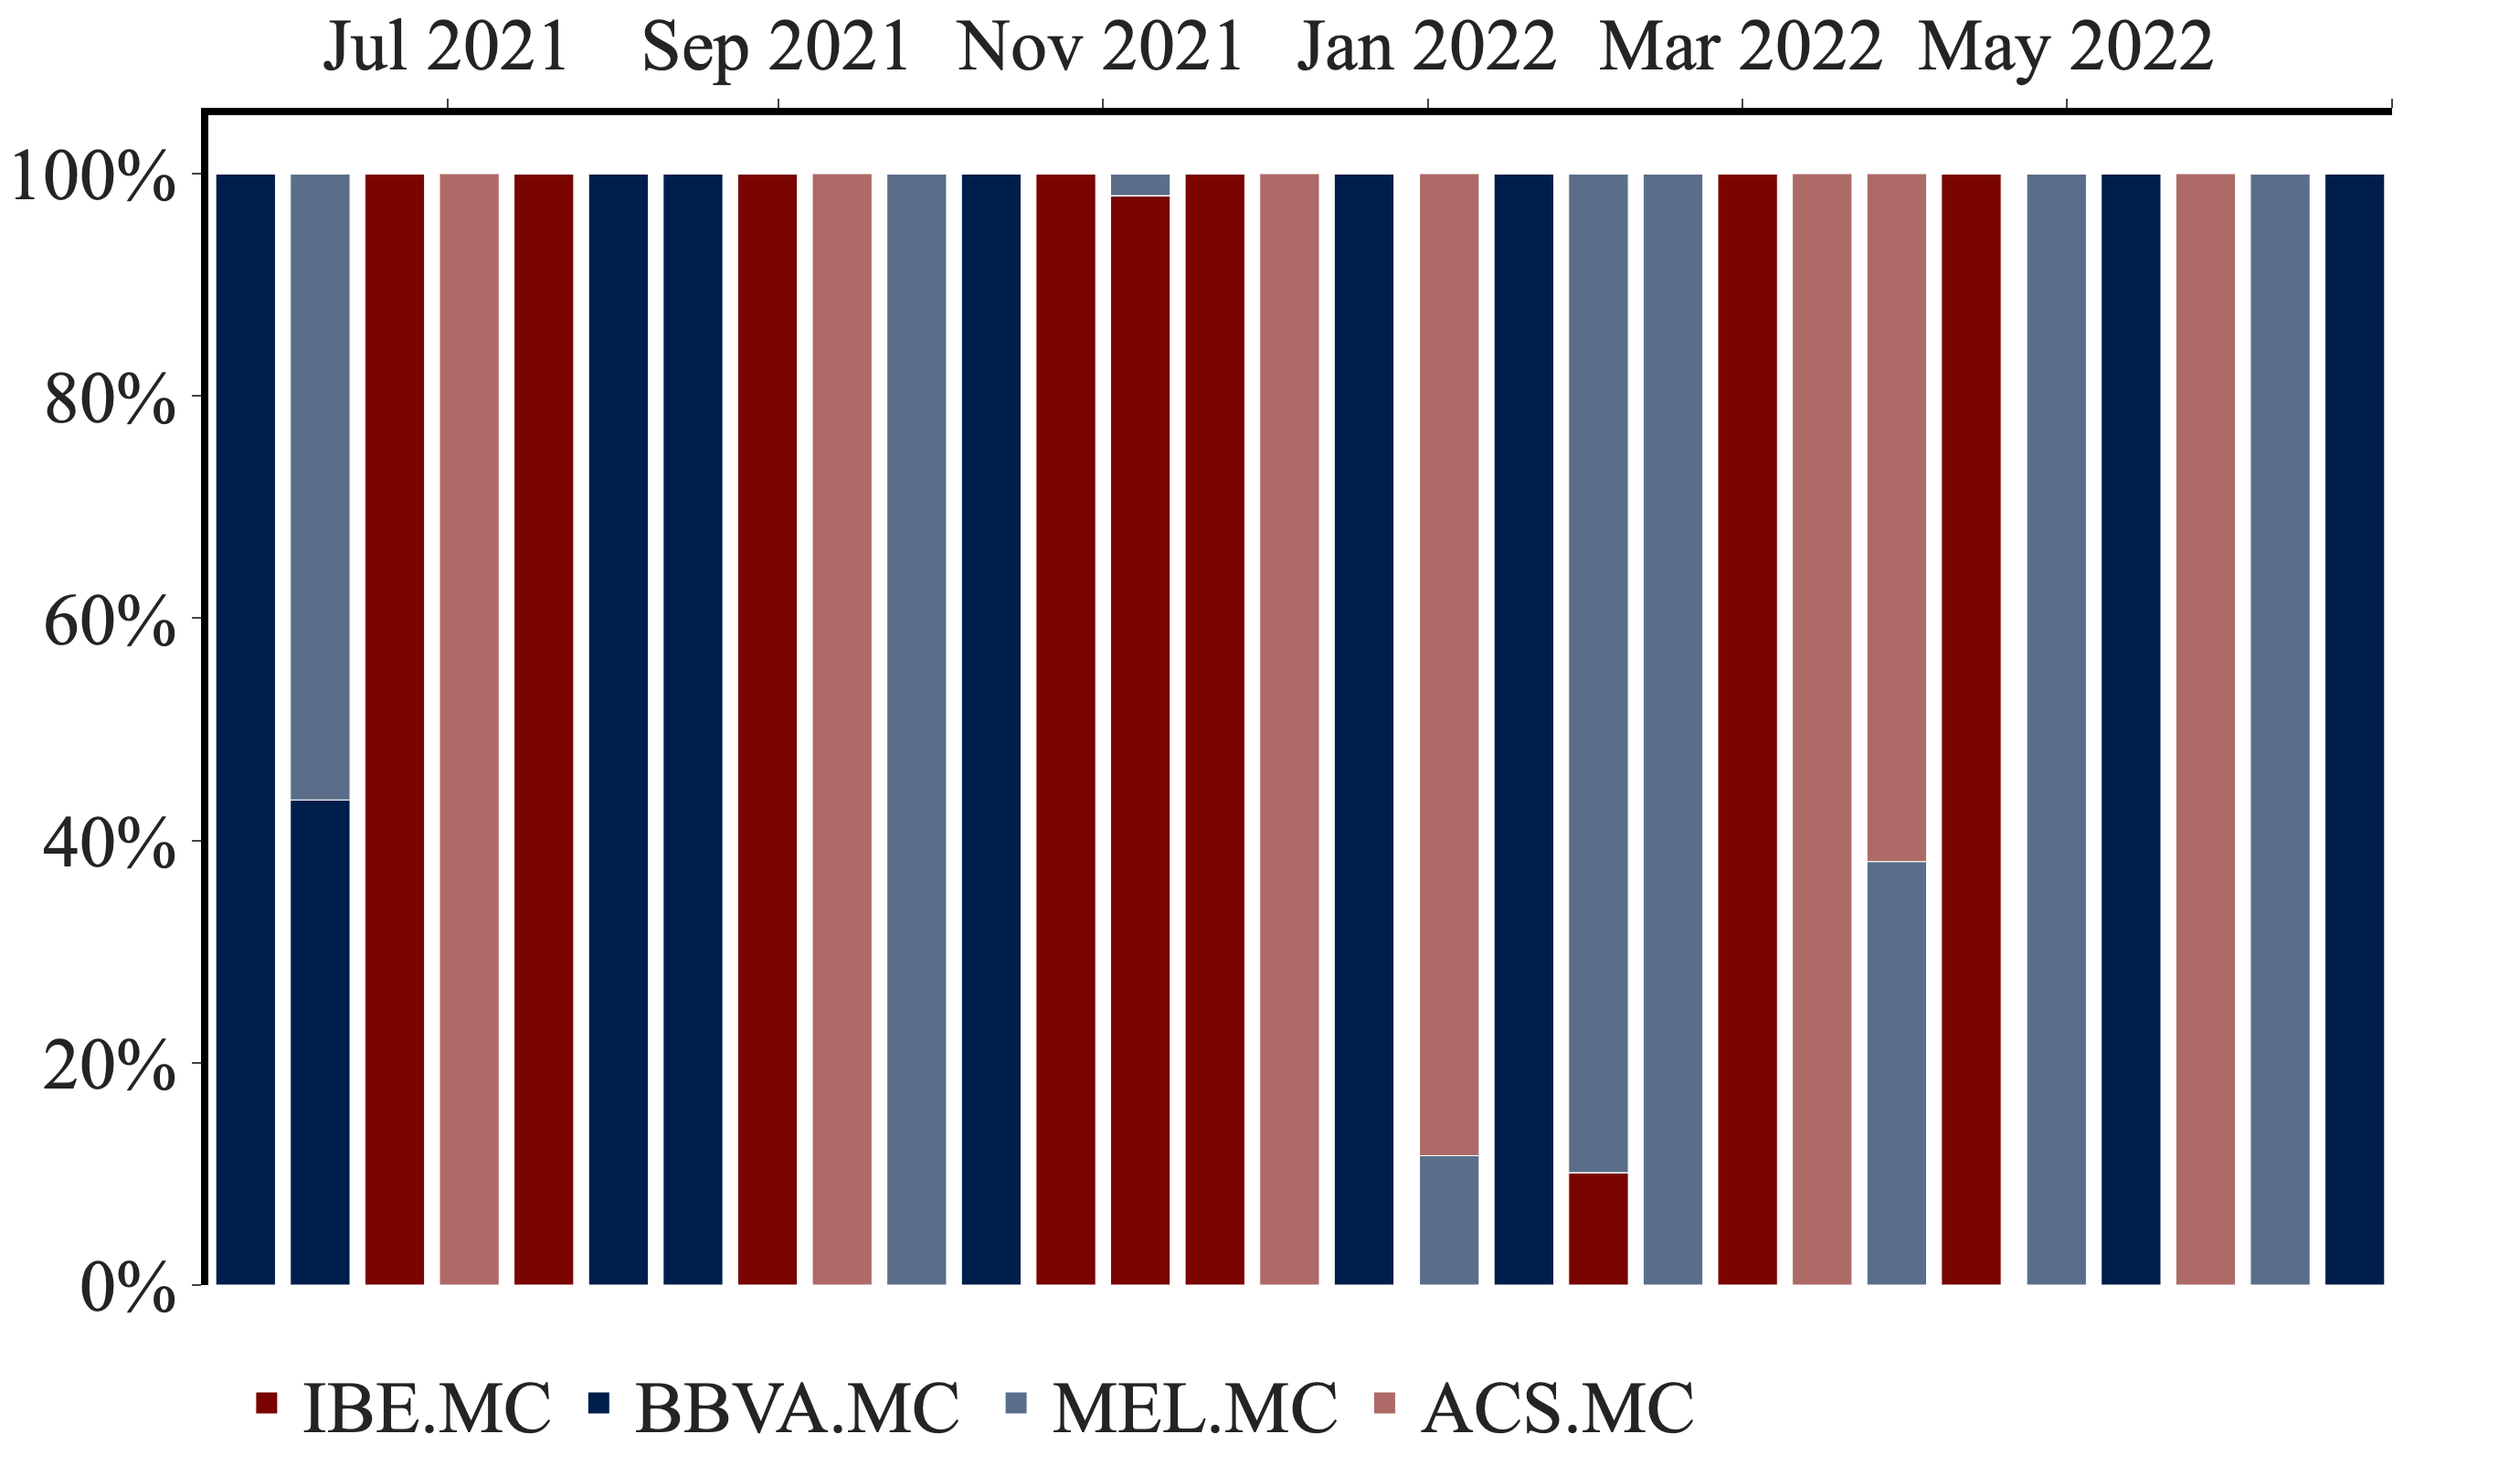
\includegraphics[width=0.4\textwidth]{Plots/w_pred.png}}}%
    \caption{Weight composition using Markowitz (left) vs deep learning Markowitz (right)}%
\end{figure}
As can be seen, the weight composition is very similar for both algorithms, only on a few rebalancings, the weights differ. The Sharpe on the portfolios can be seen below, where the figure in the left represents the 10 days Sharpe ratio and the figure in the right represents the rolling Sharpe ratio with an expanding window so that $\forall t$, $S'_{p_{t}} =\frac{1}{N} \sum_{t = 1}^{t}{S_{p_{t}}}$
\begin{figure}[H]
    \centering
{{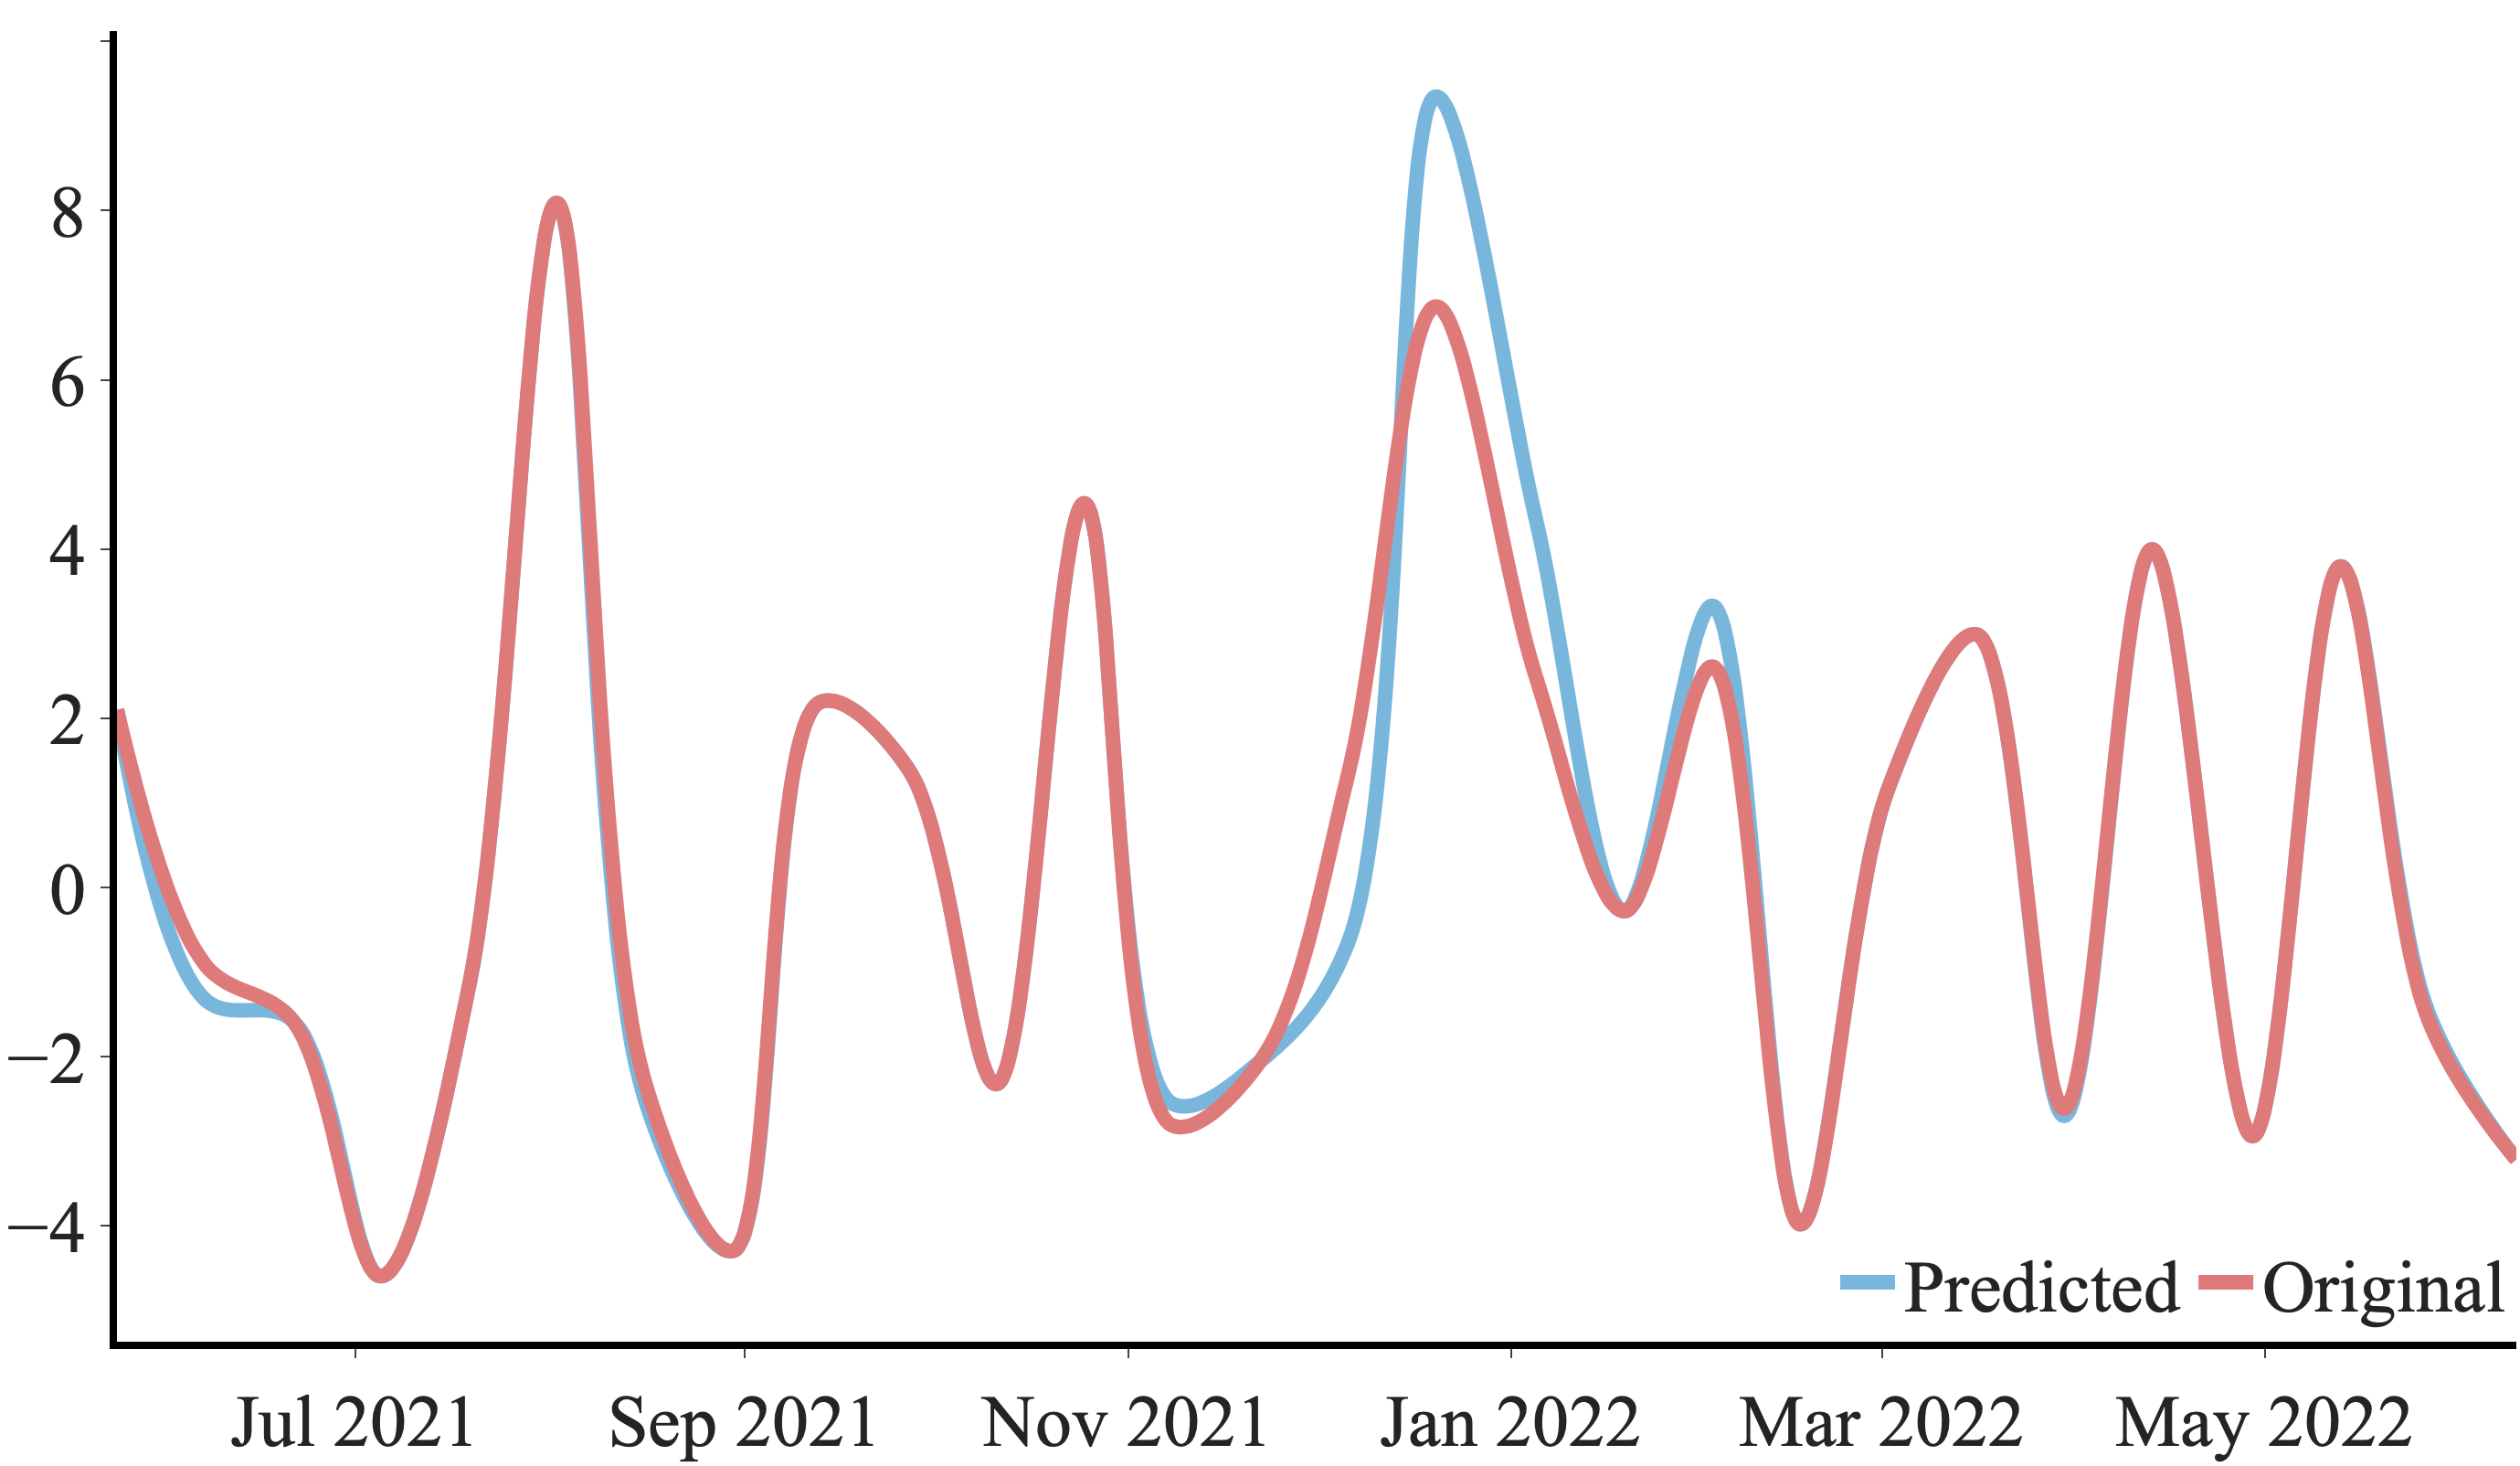
\includegraphics[width=0.4\textwidth]{Plots/sh.png}}}%
    \qquad
{{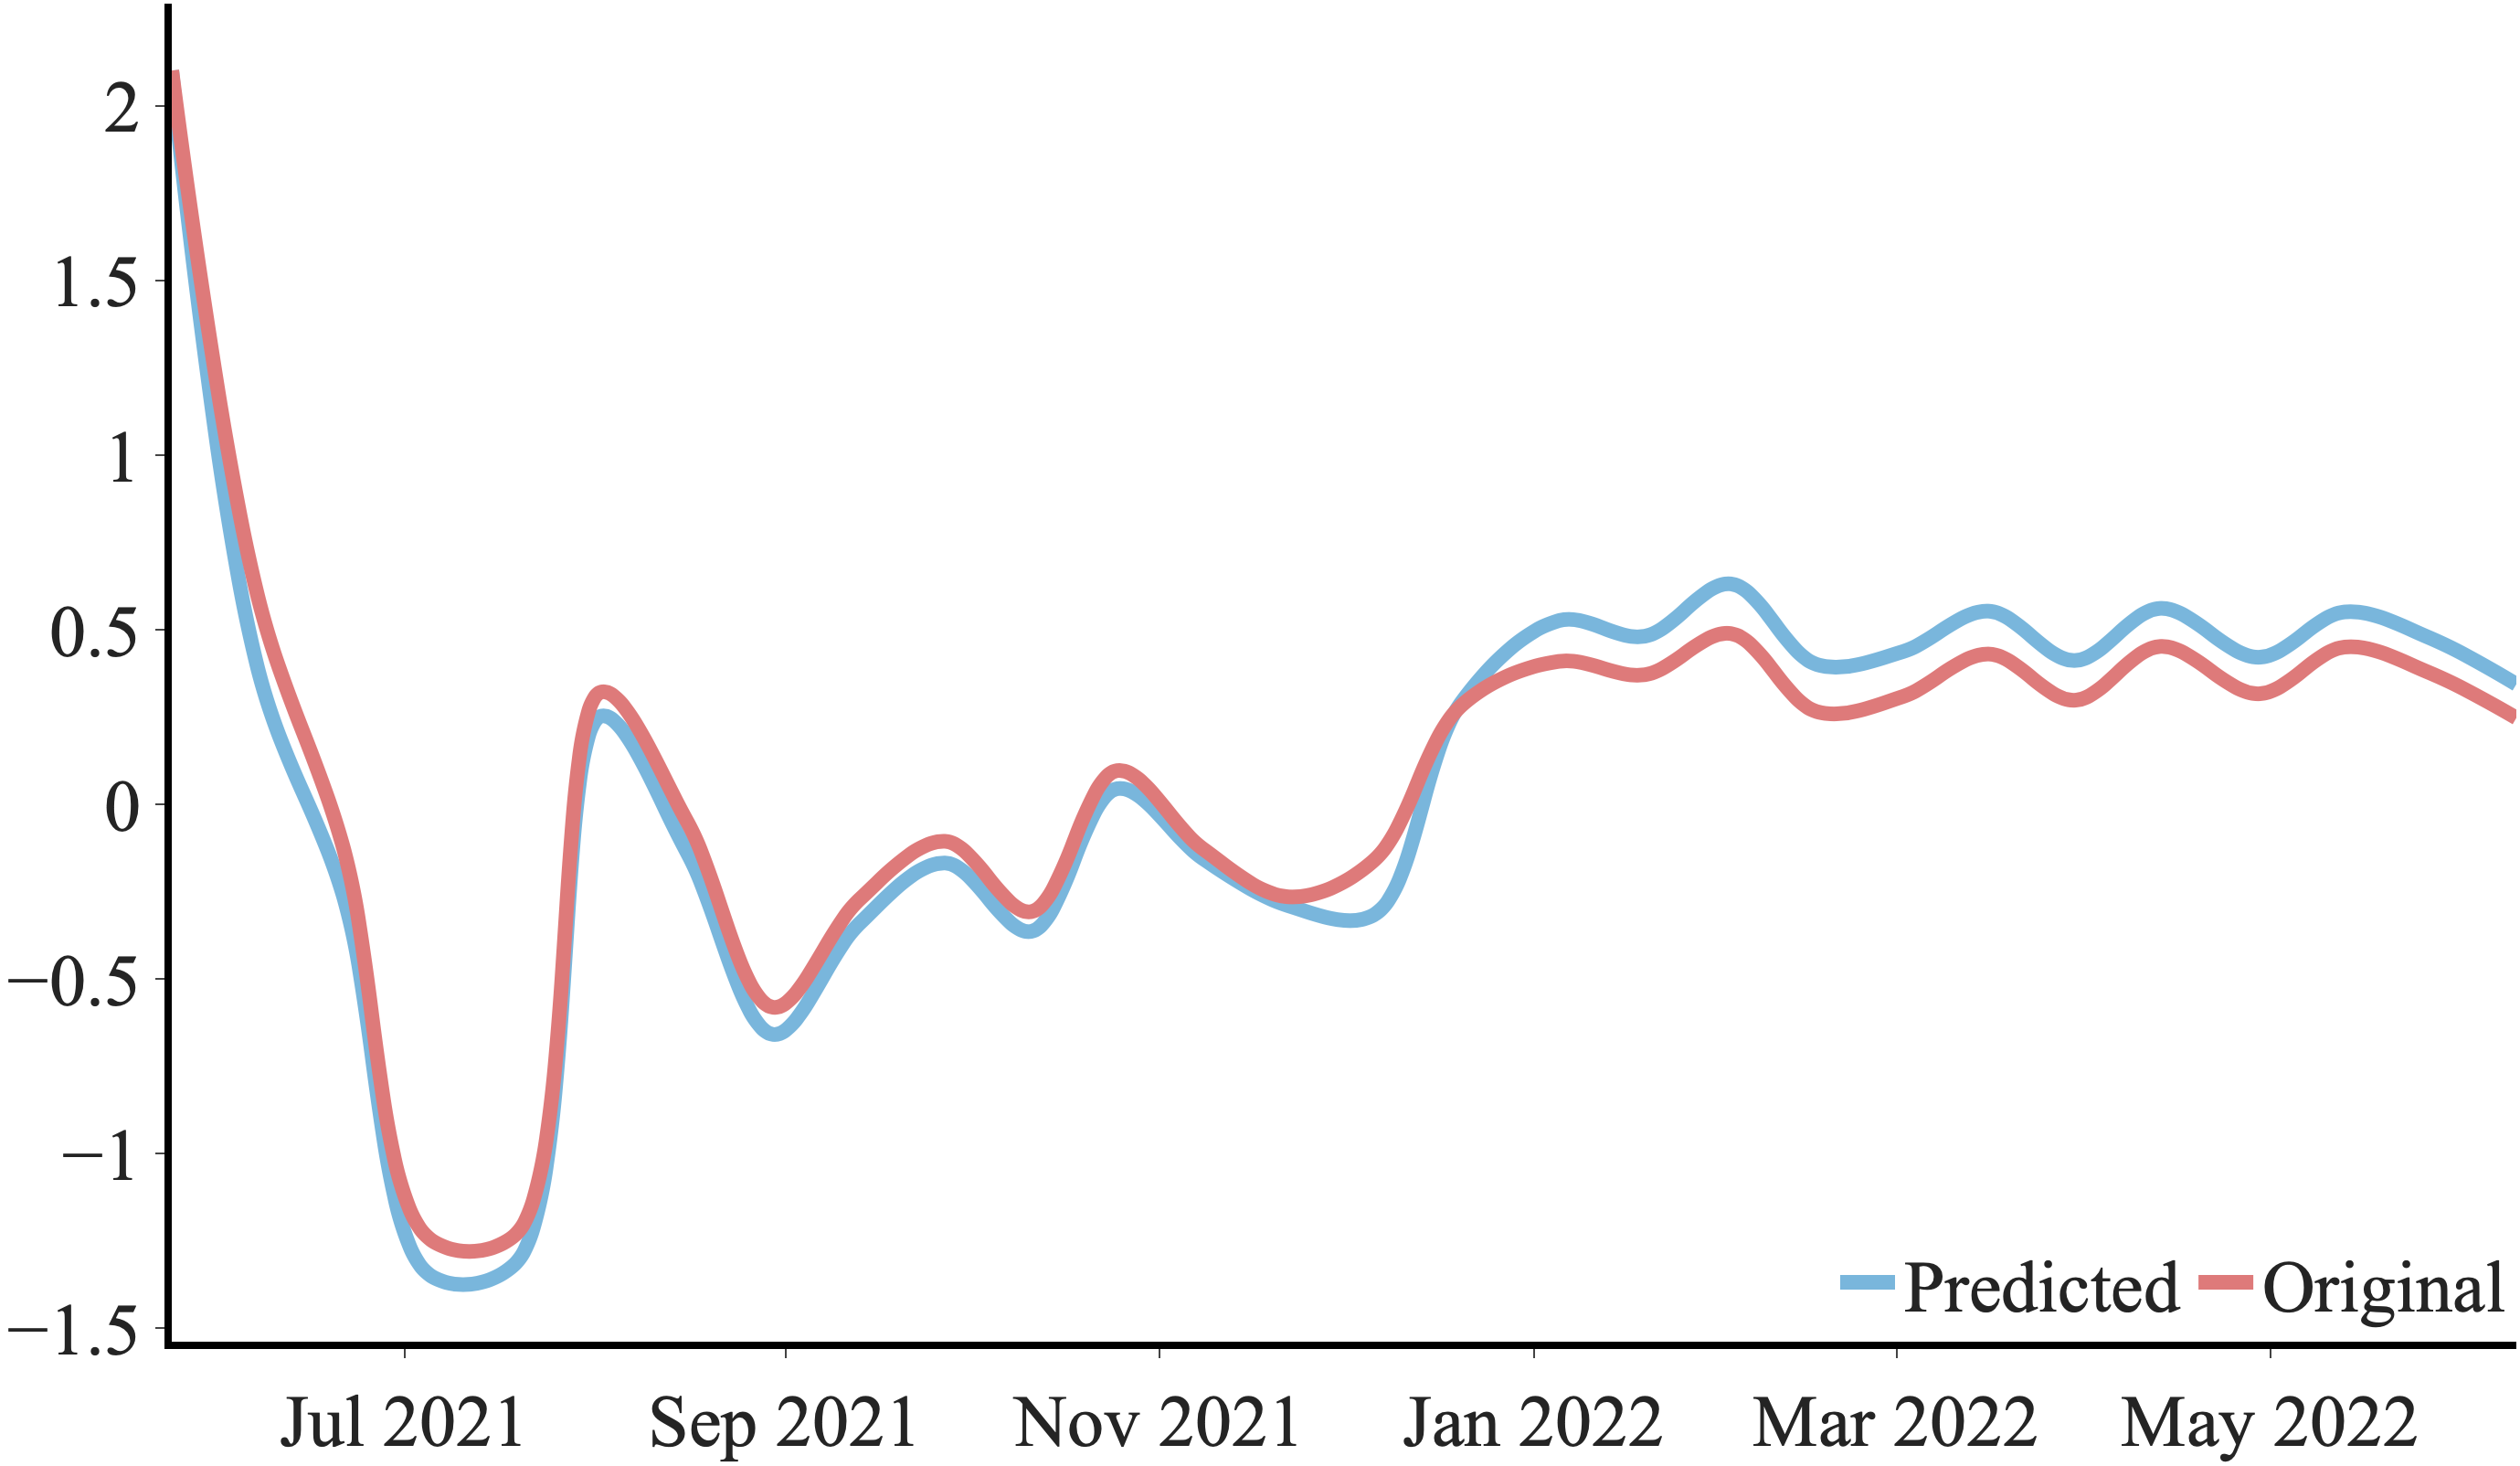
\includegraphics[width=0.4\textwidth]{Plots/sh_mean.png}}}%
    \caption{Sharpe ratio (left) vs rolling Sharpe ratio's mean (right)}%
\end{figure}

The number of positive rebalancings is 5 vs 4 negative ones, but as can be seen in the rolling mean graph, the outcome greater for \textit{boost-Marko} than for \textit{t-Marko}. This is an extended behaviour through the universe of portfolios that have been simulated. 

\section{Conclusions}
As stated in \ref{intro}, the traditional Markowitz algorithm, \textit{t-Marko}, has a main problem, the use of past information to generate portfolios expecting to maximize the mean-variance in the upcoming future.

This document has intended to prove that with the help of a predictive model, the inputs on the Markowitz model can represent better the future reality than the closest of the pasts. The use of recurrent neural networks along with convolutional neural networks has allowed us to find relationships in the temporal structure of the correlations that will help predict future behaviours.

First, it was observed that for our universe of assets, and according to the restrictions in portfolio construction, the \textit{boost-Marko} performs better more than 65\% of times. Also, it was observed that the MSE value in the training set is very correlated with the final outcome of the estimations. If the model beats the 10\% threshold, the Sharpe ratios tend to be greater in \textit{boost-Marko} than in \textit{t-Marko}, meaning that when the model is able to find the non linear correlations in the correlation cube, the predictions are normally better that the last observed values.




\bibliographystyle{alpha}
\bibliography{sample}

\end{document}